\documentclass[1p]{elsarticle_modified}
%\bibliographystyle{elsarticle-num}

%\usepackage[colorlinks]{hyperref}
%\usepackage{abbrmath_seonhwa} %\Abb, \Ascr, \Acal ,\Abf, \Afrak
\usepackage{amsfonts}
\usepackage{amssymb}
\usepackage{amsmath}
\usepackage{amsthm}
\usepackage{scalefnt}
\usepackage{amsbsy}
\usepackage{kotex}
\usepackage{caption}
\usepackage{subfig}
\usepackage{color}
\usepackage{graphicx}
\usepackage{xcolor} %% white, black, red, green, blue, cyan, magenta, yellow
\usepackage{float}
\usepackage{setspace}
\usepackage{hyperref}

\usepackage{tikz}
\usetikzlibrary{arrows}

\usepackage{multirow}
\usepackage{array} % fixed length table
\usepackage{hhline}

%%%%%%%%%%%%%%%%%%%%%
\makeatletter
\renewcommand*\env@matrix[1][\arraystretch]{%
	\edef\arraystretch{#1}%
	\hskip -\arraycolsep
	\let\@ifnextchar\new@ifnextchar
	\array{*\c@MaxMatrixCols c}}
\makeatother %https://tex.stackexchange.com/questions/14071/how-can-i-increase-the-line-spacing-in-a-matrix
%%%%%%%%%%%%%%%

\usepackage[normalem]{ulem}

\newcommand{\msout}[1]{\ifmmode\text{\sout{\ensuremath{#1}}}\else\sout{#1}\fi}
%SOURCE: \msout is \stkout macro in https://tex.stackexchange.com/questions/20609/strikeout-in-math-mode

\newcommand{\cancel}[1]{
	\ifmmode
	{\color{red}\msout{#1}}
	\else
	{\color{red}\sout{#1}}
	\fi
}

\newcommand{\add}[1]{
	{\color{blue}\uwave{#1}}
}

\newcommand{\replace}[2]{
	\ifmmode
	{\color{red}\msout{#1}}{\color{blue}\uwave{#2}}
	\else
	{\color{red}\sout{#1}}{\color{blue}\uwave{#2}}
	\fi
}

\newcommand{\Sol}{\mathcal{S}} %segment
\newcommand{\D}{D} %diagram
\newcommand{\A}{\mathcal{A}} %arc


%%%%%%%%%%%%%%%%%%%%%%%%%%%%%5 test

\def\sl{\operatorname{\textup{SL}}(2,\Cbb)}
\def\psl{\operatorname{\textup{PSL}}(2,\Cbb)}
\def\quan{\mkern 1mu \triangleright \mkern 1mu}

\theoremstyle{definition}
\newtheorem{thm}{Theorem}[section]
\newtheorem{prop}[thm]{Proposition}
\newtheorem{lem}[thm]{Lemma}
\newtheorem{ques}[thm]{Question}
\newtheorem{cor}[thm]{Corollary}
\newtheorem{defn}[thm]{Definition}
\newtheorem{exam}[thm]{Example}
\newtheorem{rmk}[thm]{Remark}
\newtheorem{alg}[thm]{Algorithm}

\newcommand{\I}{\sqrt{-1}}
\begin{document}

%\begin{frontmatter}
%
%\title{Boundary parabolic representations of knots up to 8 crossings}
%
%%% Group authors per affiliation:
%\author{Yunhi Cho} 
%\address{Department of Mathematics, University of Seoul, Seoul, Korea}
%\ead{yhcho@uos.ac.kr}
%
%
%\author{Seonhwa Kim} %\fnref{s_kim}}
%\address{Center for Geometry and Physics, Institute for Basic Science, Pohang, 37673, Korea}
%\ead{ryeona17@ibs.re.kr}
%
%\author{Hyuk Kim}
%\address{Department of Mathematical Sciences, Seoul National University, Seoul 08826, Korea}
%\ead{hyukkim@snu.ac.kr}
%
%\author{Seokbeom Yoon}
%\address{Department of Mathematical Sciences, Seoul National University, Seoul, 08826,  Korea}
%\ead{sbyoon15@snu.ac.kr}
%
%\begin{abstract}
%We find all boundary parabolic representation of knots up to 8 crossings.
%
%\end{abstract}
%\begin{keyword}
%    \MSC[2010] 57M25 
%\end{keyword}
%
%\end{frontmatter}

%\linenumbers
%\tableofcontents
%
\newcommand\colored[1]{\textcolor{white}{\rule[-0.35ex]{0.8em}{1.4ex}}\kern-0.8em\color{red} #1}%
%\newcommand\colored[1]{\textcolor{white}{ #1}\kern-2.17ex	\textcolor{white}{ #1}\kern-1.81ex	\textcolor{white}{ #1}\kern-2.15ex\color{red}#1	}

{\Large $\underline{10_{31}~(K10a_{69})}$}

\setlength{\tabcolsep}{10pt}
\renewcommand{\arraystretch}{1.6}
\vspace{1cm}\begin{tabular}{m{100pt}>{\centering\arraybackslash}m{274pt}}
\multirow{5}{120pt}{
	\centering
	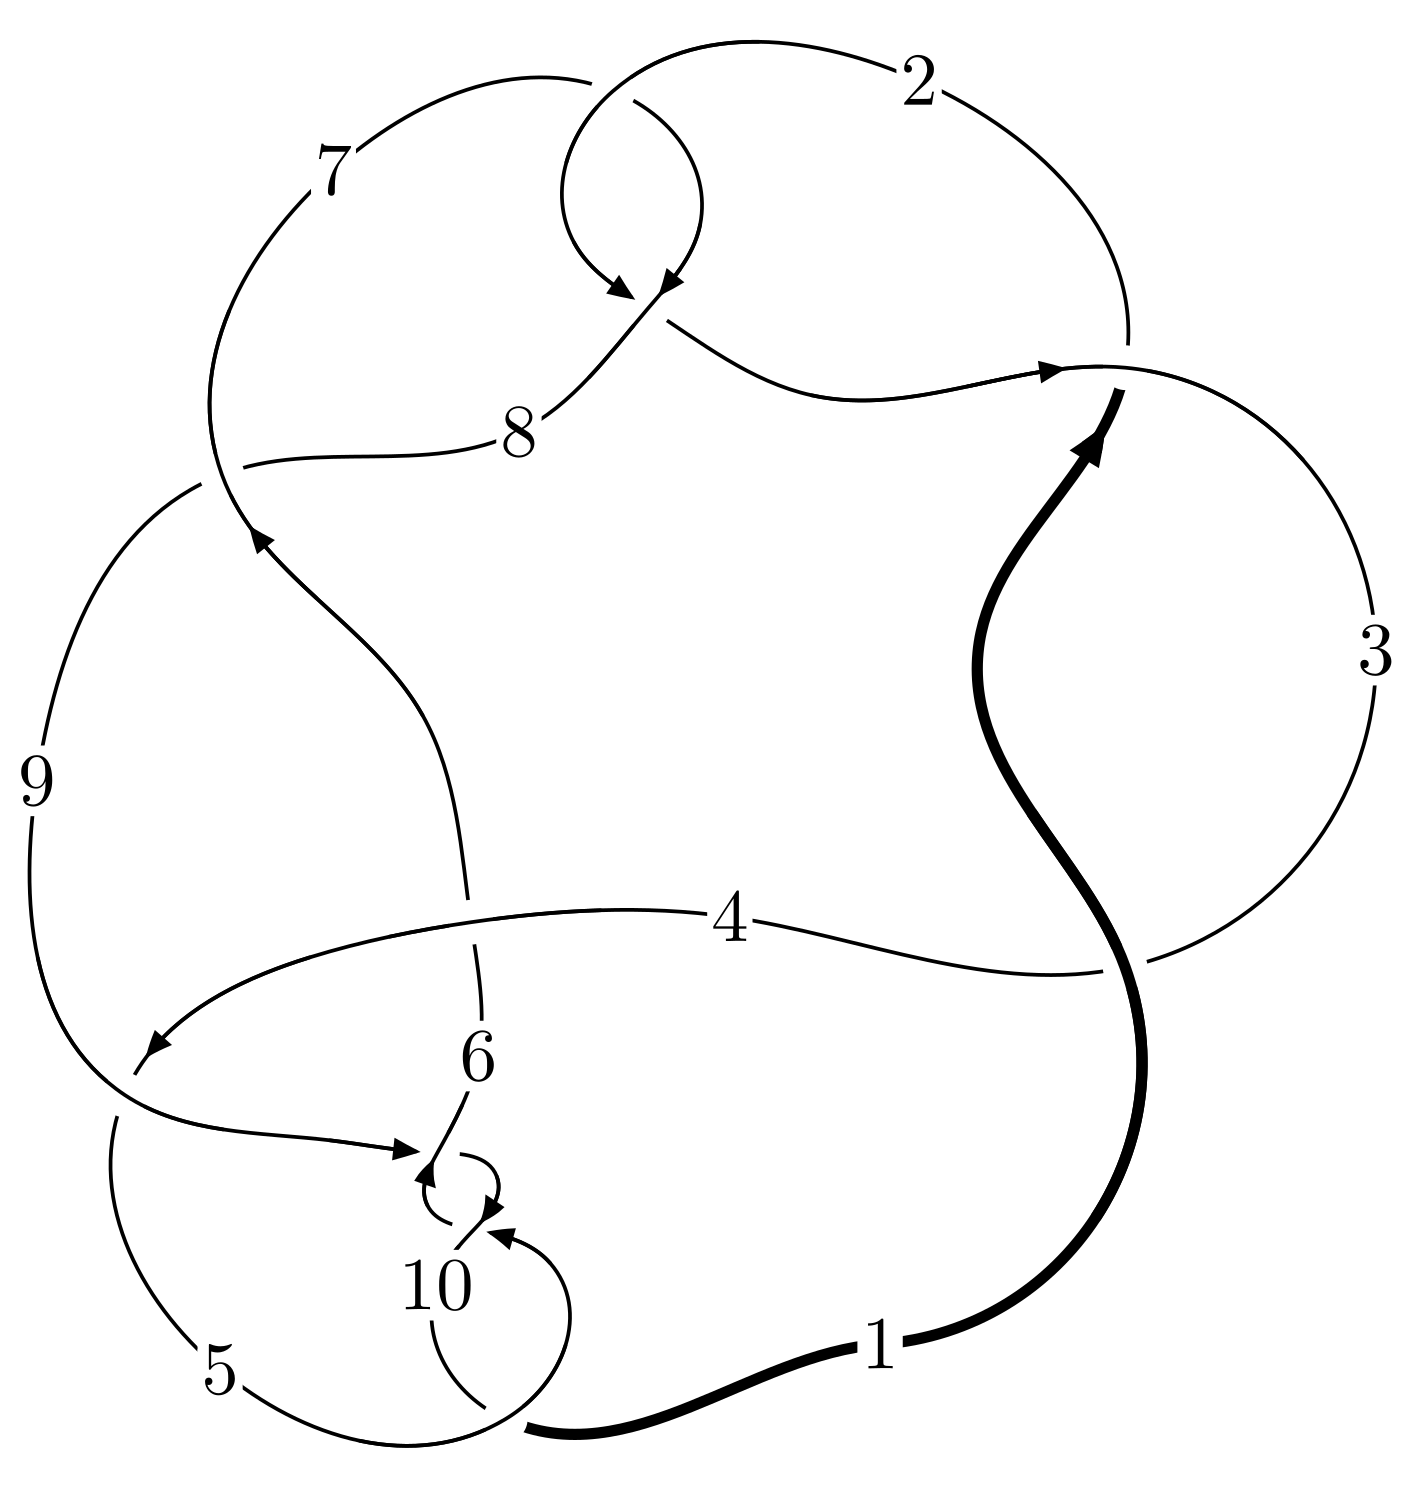
\includegraphics[width=112pt]{../../../GIT/diagram.site/Diagrams/png/115_10_31.png}\\
\ \ \ A knot diagram\footnotemark}&
\allowdisplaybreaks
\textbf{Linearized knot diagam} \\
\cline{2-2}
 &
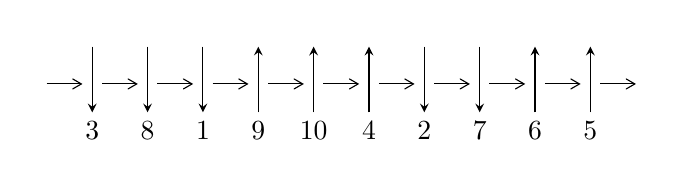
\begin{tikzpicture}[x=20pt, y=17pt]
	% nodes
	\node (C0) at (0, 0) {};
	\node (C1) at (1, 0) {};
	\node (C1U) at (1, +1) {};
	\node (C1D) at (1, -1) {3};

	\node (C2) at (2, 0) {};
	\node (C2U) at (2, +1) {};
	\node (C2D) at (2, -1) {8};

	\node (C3) at (3, 0) {};
	\node (C3U) at (3, +1) {};
	\node (C3D) at (3, -1) {1};

	\node (C4) at (4, 0) {};
	\node (C4U) at (4, +1) {};
	\node (C4D) at (4, -1) {9};

	\node (C5) at (5, 0) {};
	\node (C5U) at (5, +1) {};
	\node (C5D) at (5, -1) {10};

	\node (C6) at (6, 0) {};
	\node (C6U) at (6, +1) {};
	\node (C6D) at (6, -1) {4};

	\node (C7) at (7, 0) {};
	\node (C7U) at (7, +1) {};
	\node (C7D) at (7, -1) {2};

	\node (C8) at (8, 0) {};
	\node (C8U) at (8, +1) {};
	\node (C8D) at (8, -1) {7};

	\node (C9) at (9, 0) {};
	\node (C9U) at (9, +1) {};
	\node (C9D) at (9, -1) {6};

	\node (C10) at (10, 0) {};
	\node (C10U) at (10, +1) {};
	\node (C10D) at (10, -1) {5};
	\node (C11) at (11, 0) {};

	% arrows
	\draw[->,>={angle 60}]
	(C0) edge (C1) (C1) edge (C2) (C2) edge (C3) (C3) edge (C4) (C4) edge (C5) (C5) edge (C6) (C6) edge (C7) (C7) edge (C8) (C8) edge (C9) (C9) edge (C10) (C10) edge (C11) ;	\draw[->,>=stealth]
	(C1U) edge (C1D) (C2U) edge (C2D) (C3U) edge (C3D) (C4D) edge (C4U) (C5D) edge (C5U) (C6D) edge (C6U) (C7U) edge (C7D) (C8U) edge (C8D) (C9D) edge (C9U) (C10D) edge (C10U) ;
	\end{tikzpicture} \\
\hhline{~~} \\& 
\textbf{Solving Sequence} \\ \cline{2-2} 
 &
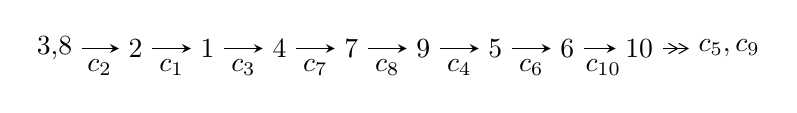
\begin{tikzpicture}[x=26pt, y=7pt]
	% node
	\node (A0) at (-1/8, 0) {3,8};
	\node (A1) at (1, 0) {2};
	\node (A2) at (2, 0) {1};
	\node (A3) at (3, 0) {4};
	\node (A4) at (4, 0) {7};
	\node (A5) at (5, 0) {9};
	\node (A6) at (6, 0) {5};
	\node (A7) at (7, 0) {6};
	\node (A8) at (8, 0) {10};
	\node (C1) at (1/2, -1) {$c_{2}$};
	\node (C2) at (3/2, -1) {$c_{1}$};
	\node (C3) at (5/2, -1) {$c_{3}$};
	\node (C4) at (7/2, -1) {$c_{7}$};
	\node (C5) at (9/2, -1) {$c_{8}$};
	\node (C6) at (11/2, -1) {$c_{4}$};
	\node (C7) at (13/2, -1) {$c_{6}$};
	\node (C8) at (15/2, -1) {$c_{10}$};
	\node (A9) at (37/4, 0) {$c_{5},c_{9}$};

	% edge
	\draw[->,>=stealth]	
	(A0) edge (A1) (A1) edge (A2) (A2) edge (A3) (A3) edge (A4) (A4) edge (A5) (A5) edge (A6) (A6) edge (A7) (A7) edge (A8) ;
	\draw[->>,>={angle 60}]	
	(A8) edge (A9);
\end{tikzpicture} \\ 

\end{tabular} \\

\footnotetext{
The image of knot diagram is generated by the software ``\textbf{Draw programme}" developed by Andrew Bartholomew(\url{http://www.layer8.co.uk/maths/draw/index.htm\#Running-draw}), where we modified some parts for our purpose(\url{https://github.com/CATsTAILs/LinksPainter}).
}\phantom \\ \newline 
\centering \textbf{Ideals for irreducible components\footnotemark of $X_{\text{par}}$} 
 
\begin{align*}
I^u_{1}&=\langle 
u^{28}- u^{27}+\cdots- u^2+1\rangle \\
\\
\end{align*}
\raggedright * 1 irreducible components of $\dim_{\mathbb{C}}=0$, with total 28 representations.\\
\footnotetext{All coefficients of polynomials are rational numbers. But the coefficients are sometimes approximated in decimal forms when there is not enough margin.}
\newpage
\renewcommand{\arraystretch}{1}
\centering \section*{I. $I^u_{1}= \langle u^{28}- u^{27}+\cdots- u^2+1 \rangle$}
\flushleft \textbf{(i) Arc colorings}\\
\begin{tabular}{m{7pt} m{180pt} m{7pt} m{180pt} }
\flushright $a_{3}=$&$\begin{pmatrix}1\\0\end{pmatrix}$ \\
\flushright $a_{8}=$&$\begin{pmatrix}0\\u\end{pmatrix}$ \\
\flushright $a_{2}=$&$\begin{pmatrix}1\\- u^2\end{pmatrix}$ \\
\flushright $a_{1}=$&$\begin{pmatrix}- u^2+1\\- u^2\end{pmatrix}$ \\
\flushright $a_{4}=$&$\begin{pmatrix}u^4- u^2+1\\u^4\end{pmatrix}$ \\
\flushright $a_{7}=$&$\begin{pmatrix}u\\- u^3+u\end{pmatrix}$ \\
\flushright $a_{9}=$&$\begin{pmatrix}- u^3\\u^5- u^3+u\end{pmatrix}$ \\
\flushright $a_{5}=$&$\begin{pmatrix}u^{12}- u^{10}+3 u^8-2 u^6+2 u^4- u^2+1\\- u^{14}+2 u^{12}-5 u^{10}+6 u^8-6 u^6+4 u^4- u^2\end{pmatrix}$ \\
\flushright $a_{6}=$&$\begin{pmatrix}u^{11}-2 u^9+4 u^7-4 u^5+3 u^3\\u^{11}- u^9+2 u^7- u^5- u^3+u\end{pmatrix}$ \\
\flushright $a_{10}=$&$\begin{pmatrix}u^{27}-4 u^{25}+\cdots+12 u^7- u^3\\u^{27}-3 u^{25}+\cdots- u^3+u\end{pmatrix}$\\&\end{tabular}
\flushleft \textbf{(ii) Obstruction class $= -1$}\\~\\
\flushleft \textbf{(iii) Cusp Shapes $= 4 u^{26}-4 u^{25}-12 u^{24}+16 u^{23}+44 u^{22}-52 u^{21}-88 u^{20}+116 u^{19}+168 u^{18}-204 u^{17}-236 u^{16}+284 u^{15}+288 u^{14}-312 u^{13}-280 u^{12}+256 u^{11}+224 u^{10}-152 u^9-136 u^8+40 u^7+64 u^6+16 u^5-16 u^4-16 u^3+4 u-2$}\\~\\
\newpage\renewcommand{\arraystretch}{1}
\flushleft \textbf{(iv) u-Polynomials at the component}\newline \\
\begin{tabular}{m{50pt}|m{274pt}}
Crossings & \hspace{64pt}u-Polynomials at each crossing \\
\hline $$\begin{aligned}c_{1},c_{3},c_{8}\end{aligned}$$&$\begin{aligned}
&u^{28}+7 u^{27}+\cdots+2 u+1
\end{aligned}$\\
\hline $$\begin{aligned}c_{2},c_{7}\end{aligned}$$&$\begin{aligned}
&u^{28}- u^{27}+\cdots- u^2+1
\end{aligned}$\\
\hline $$\begin{aligned}c_{4}\end{aligned}$$&$\begin{aligned}
&u^{28}- u^{27}+\cdots+5 u+2
\end{aligned}$\\
\hline $$\begin{aligned}c_{5},c_{9},c_{10}\end{aligned}$$&$\begin{aligned}
&u^{28}+u^{27}+\cdots+2 u+1
\end{aligned}$\\
\hline $$\begin{aligned}c_{6}\end{aligned}$$&$\begin{aligned}
&u^{28}+7 u^{27}+\cdots+8 u+1
\end{aligned}$\\
\hline
\end{tabular}\\~\\
\newpage\renewcommand{\arraystretch}{1}
\flushleft \textbf{(v) Riley Polynomials at the component}\newline \\
\begin{tabular}{m{50pt}|m{274pt}}
Crossings & \hspace{64pt}Riley Polynomials at each crossing \\
\hline $$\begin{aligned}c_{1},c_{3},c_{8}\end{aligned}$$&$\begin{aligned}
&y^{28}+29 y^{27}+\cdots+14 y+1
\end{aligned}$\\
\hline $$\begin{aligned}c_{2},c_{7}\end{aligned}$$&$\begin{aligned}
&y^{28}-7 y^{27}+\cdots-2 y+1
\end{aligned}$\\
\hline $$\begin{aligned}c_{4}\end{aligned}$$&$\begin{aligned}
&y^{28}-3 y^{27}+\cdots+19 y+4
\end{aligned}$\\
\hline $$\begin{aligned}c_{5},c_{9},c_{10}\end{aligned}$$&$\begin{aligned}
&y^{28}+25 y^{27}+\cdots-2 y+1
\end{aligned}$\\
\hline $$\begin{aligned}c_{6}\end{aligned}$$&$\begin{aligned}
&y^{28}+y^{27}+\cdots+62 y+1
\end{aligned}$\\
\hline
\end{tabular}\\~\\
\newpage\flushleft \textbf{(vi) Complex Volumes and Cusp Shapes}
$$\begin{array}{c|c|c}  
\text{Solutions to }I^u_{1}& \I (\text{vol} + \sqrt{-1}CS) & \text{Cusp shape}\\
 \hline 
\begin{aligned}
u &= \phantom{-}0.899770 + 0.359295 I\end{aligned}
 & -0.52966 - 3.76187 I & -0.54869 + 7.99757 I \\ \hline\begin{aligned}
u &= \phantom{-}0.899770 - 0.359295 I\end{aligned}
 & -0.52966 + 3.76187 I & -0.54869 - 7.99757 I \\ \hline\begin{aligned}
u &= \phantom{-}0.954301 + 0.165131 I\end{aligned}
 & -6.93655 + 1.29573 I & -8.16340 + 0.19021 I \\ \hline\begin{aligned}
u &= \phantom{-}0.954301 - 0.165131 I\end{aligned}
 & -6.93655 - 1.29573 I & -8.16340 - 0.19021 I \\ \hline\begin{aligned}
u &= -0.971170 + 0.356128 I\end{aligned}
 & -5.84563 + 6.87695 I & -5.38448 - 7.29150 I \\ \hline\begin{aligned}
u &= -0.971170 - 0.356128 I\end{aligned}
 & -5.84563 - 6.87695 I & -5.38448 + 7.29150 I \\ \hline\begin{aligned}
u &= -0.816311 + 0.219669 I\end{aligned}
 & -1.41378 + 0.68499 I & -4.66956 - 0.56233 I \\ \hline\begin{aligned}
u &= -0.816311 - 0.219669 I\end{aligned}
 & -1.41378 - 0.68499 I & -4.66956 + 0.56233 I \\ \hline\begin{aligned}
u &= -0.894569 + 0.739690 I\end{aligned}
 & -1.93517 + 2.81005 I & -2.61718 - 2.93426 I \\ \hline\begin{aligned}
u &= -0.894569 - 0.739690 I\end{aligned}
 & -1.93517 - 2.81005 I & -2.61718 + 2.93426 I \\ \hline\begin{aligned}
u &= -0.594944 + 0.540484 I\end{aligned}
 & -1.95488 + 1.97473 I & \phantom{-}0.55963 - 3.90307 I \\ \hline\begin{aligned}
u &= -0.594944 - 0.540484 I\end{aligned}
 & -1.95488 - 1.97473 I & \phantom{-}0.55963 + 3.90307 I \\ \hline\begin{aligned}
u &= \phantom{-}0.824272 + 0.873080 I\end{aligned}
 & \phantom{-}2.07406 + 4.77850 I & \phantom{-}0.63399 - 2.38985 I \\ \hline\begin{aligned}
u &= \phantom{-}0.824272 - 0.873080 I\end{aligned}
 & \phantom{-}2.07406 - 4.77850 I & \phantom{-}0.63399 + 2.38985 I \\ \hline\begin{aligned}
u &= -0.848977 + 0.862822 I\end{aligned}
 & \phantom{-}7.13238 - 0.98573 I & \phantom{-}5.20004 + 1.21736 I \\ \hline\begin{aligned}
u &= -0.848977 - 0.862822 I\end{aligned}
 & \phantom{-}7.13238 + 0.98573 I & \phantom{-}5.20004 - 1.21736 I \\ \hline\begin{aligned}
u &= \phantom{-}0.883885 + 0.841772 I\end{aligned}
 & \phantom{-}4.95278 - 2.93440 I & \phantom{-}2.09657 + 3.53352 I \\ \hline\begin{aligned}
u &= \phantom{-}0.883885 - 0.841772 I\end{aligned}
 & \phantom{-}4.95278 + 2.93440 I & \phantom{-}2.09657 - 3.53352 I \\ \hline\begin{aligned}
u &= \phantom{-}0.921489 + 0.824235 I\end{aligned}
 & \phantom{-}4.83159 - 3.27187 I & \phantom{-}1.73251 + 1.59380 I \\ \hline\begin{aligned}
u &= \phantom{-}0.921489 - 0.824235 I\end{aligned}
 & \phantom{-}4.83159 + 3.27187 I & \phantom{-}1.73251 - 1.59380 I \\ \hline\begin{aligned}
u &= -0.956709 + 0.821698 I\end{aligned}
 & \phantom{-}6.79399 + 7.24627 I & \phantom{-}4.35343 - 6.30493 I \\ \hline\begin{aligned}
u &= -0.956709 - 0.821698 I\end{aligned}
 & \phantom{-}6.79399 - 7.24627 I & \phantom{-}4.35343 + 6.30493 I \\ \hline\begin{aligned}
u &= \phantom{-}0.975960 + 0.814541 I\end{aligned}
 & \phantom{-}1.59839 - 11.04430 I & -0.28365 + 7.20583 I \\ \hline\begin{aligned}
u &= \phantom{-}0.975960 - 0.814541 I\end{aligned}
 & \phantom{-}1.59839 + 11.04430 I & -0.28365 - 7.20583 I \\ \hline\begin{aligned}
u &= -0.190095 + 0.611771 I\end{aligned}
 & -3.43315 - 3.38176 I & \phantom{-}0.34958 + 2.75424 I \\ \hline\begin{aligned}
u &= -0.190095 - 0.611771 I\end{aligned}
 & -3.43315 + 3.38176 I & \phantom{-}0.34958 - 2.75424 I \\ \hline\begin{aligned}
u &= \phantom{-}0.313097 + 0.488114 I\end{aligned}
 & \phantom{-}1.245360 + 0.507461 I & \phantom{-}6.74123 - 1.23953 I \\ \hline\begin{aligned}
u &= \phantom{-}0.313097 - 0.488114 I\end{aligned}
 & \phantom{-}1.245360 - 0.507461 I & \phantom{-}6.74123 + 1.23953 I\\
 \hline 
 \end{array}$$\newpage
\newpage\renewcommand{\arraystretch}{1}
\centering \section*{ II. u-Polynomials}
\begin{tabular}{m{50pt}|m{274pt}}
Crossings & \hspace{64pt}u-Polynomials at each crossing \\
\hline $$\begin{aligned}c_{1},c_{3},c_{8}\end{aligned}$$&$\begin{aligned}
&u^{28}+7 u^{27}+\cdots+2 u+1
\end{aligned}$\\
\hline $$\begin{aligned}c_{2},c_{7}\end{aligned}$$&$\begin{aligned}
&u^{28}- u^{27}+\cdots- u^2+1
\end{aligned}$\\
\hline $$\begin{aligned}c_{4}\end{aligned}$$&$\begin{aligned}
&u^{28}- u^{27}+\cdots+5 u+2
\end{aligned}$\\
\hline $$\begin{aligned}c_{5},c_{9},c_{10}\end{aligned}$$&$\begin{aligned}
&u^{28}+u^{27}+\cdots+2 u+1
\end{aligned}$\\
\hline $$\begin{aligned}c_{6}\end{aligned}$$&$\begin{aligned}
&u^{28}+7 u^{27}+\cdots+8 u+1
\end{aligned}$\\
\hline
\end{tabular}\newpage\renewcommand{\arraystretch}{1}
\centering \section*{ III. Riley Polynomials}
\begin{tabular}{m{50pt}|m{274pt}}
Crossings & \hspace{64pt}Riley Polynomials at each crossing \\
\hline $$\begin{aligned}c_{1},c_{3},c_{8}\end{aligned}$$&$\begin{aligned}
&y^{28}+29 y^{27}+\cdots+14 y+1
\end{aligned}$\\
\hline $$\begin{aligned}c_{2},c_{7}\end{aligned}$$&$\begin{aligned}
&y^{28}-7 y^{27}+\cdots-2 y+1
\end{aligned}$\\
\hline $$\begin{aligned}c_{4}\end{aligned}$$&$\begin{aligned}
&y^{28}-3 y^{27}+\cdots+19 y+4
\end{aligned}$\\
\hline $$\begin{aligned}c_{5},c_{9},c_{10}\end{aligned}$$&$\begin{aligned}
&y^{28}+25 y^{27}+\cdots-2 y+1
\end{aligned}$\\
\hline $$\begin{aligned}c_{6}\end{aligned}$$&$\begin{aligned}
&y^{28}+y^{27}+\cdots+62 y+1
\end{aligned}$\\
\hline
\end{tabular}
\vskip 2pc
\end{document}